\subsection{Simulation in COMSOL}

\subsubsection{Motivation for synthetic simulation}

For the task of AI-based prediction of thermoelastic wave propagation in geological media, a suitable open dataset was not found. Most available open datasets are not designed for coupled thermo-mechanical modelling in a two-dimensional geological medium. In particular, they usually do not contain a complete combination of two-dimensional geological geometry, transient thermal fields, displacement fields, strain fields, stress distributions, material parameters of different rocks, and mesh-based spatial structure suitable for graph-based neural networks. Therefore, the generation of a synthetic dataset using numerical simulation was selected as the most controllable and physically consistent approach.

Before selecting the final simulation environment, several software tools were considered. ANSYS was considered as a powerful finite element analysis environment. However, the regular generation of many two-dimensional coupled thermo-mechanical simulations required higher computational resources and a more complex simulation pipeline than was available in this project. NVIDIA Omniverse was also considered as a modern platform for visualization and physically realistic scenes. However, the main goal of this work was not only visualization, but also numerical extraction of temperature, displacement, strain, and stress fields. For this reason, Omniverse was less suitable as the main source of ground-truth simulation data.

COMSOL Multiphysics was selected as an engineering decision under computational limitations. It provides a convenient environment for multiphysics coupling, finite element modelling, time-dependent solvers, material definition, boundary condition assignment, visualization, and export of numerical fields. This made it suitable for generating a controlled synthetic dataset for the later machine learning stages.

\subsubsection{Geometry of the thermoelastic experiment}

\begin{figure}[h]
\centering
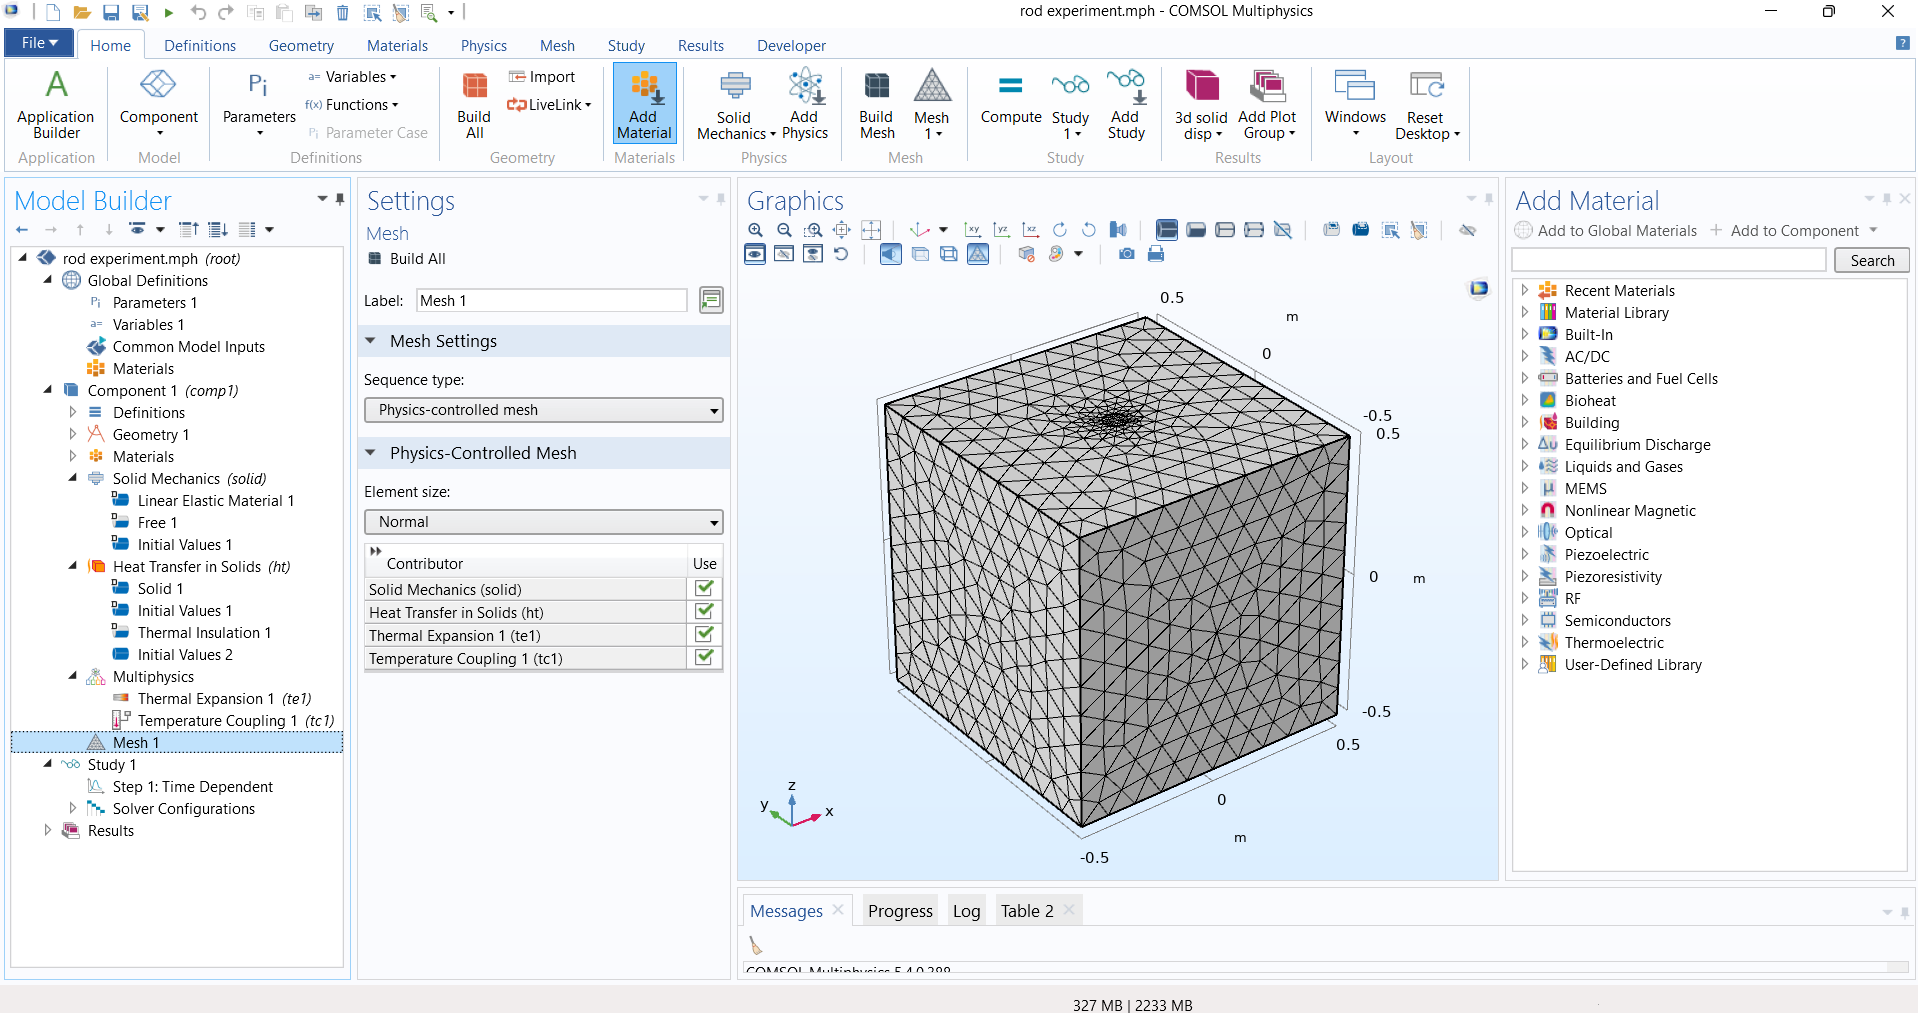
\includegraphics[width=0.8\textwidth]{chapters/chapter4/interface.png}
\caption{interface of Comsol Multiphysics}
\end{figure}

The simulated physical system consists of a two-dimensional rock domain and a heated metallic rod partially inserted into the rock. The rock represents the geological medium, while the rod acts as a localized thermal excitation source. The size of the rock domain is denoted as

\[
L_x \times L_y \times L_z.
\]

The radius of the inserted rod is denoted by

\[
R_{\mathrm{rod}},
\]

and the penetration depth of the rod into the rock is denoted by

\[
d_{\mathrm{rod}}.
\]

The initial temperature of the rock is denoted by \(T_0\), while the initial temperature of the rod is denoted by \(T_{\mathrm{rod}}\). In the considered experiment, the rod is hotter than the surrounding rock:

\[
T_{\mathrm{rod}} > T_0.
\]

The heated rod creates a localized temperature disturbance. Heat propagates from the rod into the surrounding geological medium by conduction. Since the temperature distribution inside the rock is non-uniform, different parts of the material expand by different amounts. This produces thermal strain, mechanical stress, and displacement fields. In a time-dependent formulation, the mechanical response appears as a propagating thermoelastic disturbance through the rock volume.

The computational domain is written as

\[
\Omega =
\Omega_{\mathrm{rock}}
\cup
\Omega_{\mathrm{rod}},
\]

where \(\Omega_{\mathrm{rock}}\) is the rock domain and \(\Omega_{\mathrm{rod}}\) is the rod domain. In COMSOL, these domains are assigned different material properties. This is important because the thermal and mechanical response of metal and rock are different.

\subsubsection{Physical interfaces used in COMSOL}

The COMSOL model was configured as a coupled thermo-mechanical simulation. The physical interfaces can be grouped into four main parts.

The first part is the thermal physics. The \textit{Heat Transfer in Solids} interface was used to solve transient heat conduction in both the rock and the rod. This interface computes the temperature field \(T(x,t)\) over the computational domain.

The second part is the structural mechanics. The \textit{Solid Mechanics} interface was used to compute displacement, strain, and stress caused by thermal expansion and dynamic mechanical response. The displacement field is obtained as a function of space and time.

The third part is the multiphysics coupling. The \textit{Thermal Expansion} coupling transfers the temperature field from the heat transfer interface to the solid mechanics interface. The temperature change produces thermal strain, which is included in the mechanical formulation.

The fourth part is the time-dependent study. The coupled system is solved over a time interval, producing a sequence of physical fields at multiple time steps. Therefore, the output of the COMSOL model is not a single static solution, but a time-dependent sequence of thermoelastic states.
\subsubsection{Heat transfer formulation}

The heat transfer process is based on Fourier's law:

\[
q = -k \nabla T,
\]

where \(q\) is the heat flux vector, \(k\) is the thermal conductivity, and \(T\) is the temperature field. The negative sign means that heat flows from hotter regions to colder regions. Therefore, the heat flux is directed opposite to the temperature gradient.

The transient heat conduction equation is written as

\[
\rho C_p \frac{\partial T}{\partial t}
=
\nabla \cdot \left( k \nabla T \right) + Q,
\]

where \(\rho\) is the material density, \(C_p\) is the heat capacity at constant pressure, \(t\) is time, and \(Q\) is the volumetric heat source. The left-hand side describes the accumulation of thermal energy inside the material. The first term on the right-hand side describes heat conduction, while \(Q\) represents internal or external heat generation.

In this experiment, the heated rod acts as the main source of thermal disturbance. Depending on the simulation setup, the rod can be represented either by an initial high temperature or by a prescribed heat source term. Since the rock and the rod are different materials, their thermal properties are spatially dependent:

\[
\rho = \rho(x), \qquad
C_p = C_p(x), \qquad
k = k(x),
\]

where

\[
x = (x, y).
\]

This means that the heat equation is solved with different material parameters in the rock and in the metallic rod.

\subsubsection{Solid mechanics formulation}

The mechanical response of the rock is described using the displacement vector

\[
u(x,t)
=
\begin{bmatrix}
u(x,t) \\
v(x,t) \\
w(x,t)
\end{bmatrix},
\]

where \(u\), \(v\), and \(w\) are displacement components along the \(x\), \(y\), and \(z\) axes. For small deformations, the strain tensor is defined as

\[
\varepsilon
=
\frac{1}{2}
\left(
\nabla u
+
(\nabla u)^{T}
\right).
\]

This tensor describes local deformation caused by mechanical displacement. In a thermoelastic problem, deformation is caused not only by mechanical loading, but also by temperature change. The thermal strain is expressed as

\[
\varepsilon_{\mathrm{th}}
=
\alpha
\left(
T - T_{\mathrm{ref}}
\right)
I,
\]

where \(\alpha\) is the coefficient of thermal expansion, \(T_{\mathrm{ref}}\) is the reference temperature, and \(I\) is the identity tensor. Thermal strain describes expansion or contraction of the material due to heating or cooling.

The elastic strain is the part of the total strain that contributes to mechanical stress:

\[
\varepsilon_{\mathrm{el}}
=
\varepsilon
-
\varepsilon_{\mathrm{th}}.
\]

The constitutive relation between stress and elastic strain is written as

\[
\sigma
=
C
:
\left(
\varepsilon
-
\varepsilon_{\mathrm{th}}
\right),
\]

where \(\sigma\) is the Cauchy stress tensor and \(C\) is the elasticity tensor. For an isotropic linear elastic material, this relation can be written as

\[
\sigma
=
\lambda \,
\mathrm{tr}
\left(
\varepsilon_{\mathrm{el}}
\right)
I
+
2 \mu
\varepsilon_{\mathrm{el}},
\]

where \(\lambda\) and \(\mu\) are Lamé parameters:

\[
\lambda =
\frac{E \nu}
{(1+\nu)(1-2\nu)},
\qquad
\mu =
\frac{E}{2(1+\nu)}.
\]

Here, \(E\) is Young's modulus and \(\nu\) is Poisson's ratio. Young's modulus defines the stiffness of the material, while Poisson's ratio describes lateral deformation under loading.

The dynamic mechanical response is governed by the equation of motion:

\[
\rho
\frac{\partial^2 u}{\partial t^2}
=
\nabla \cdot \sigma
+
f,
\]

where \(\rho\) is the density and \(f\) is the body force vector. This equation describes how stress gradients produce acceleration of the material. The divergence of the stress tensor acts as an internal force, while the inertial term controls wave-like propagation of displacement.

\subsubsection{Thermoelastic coupling}

The thermoelastic coupling is the central physical mechanism of the simulation. The heat transfer interface computes the temperature field \(T(x,t)\). This temperature field is then passed to the solid mechanics interface. COMSOL uses the temperature difference relative to the reference temperature to compute the thermal strain:

\[
\varepsilon_{\mathrm{th}}
=
\alpha
\left(
T - T_{\mathrm{ref}}
\right)
I.
\]

The thermal strain modifies the elastic strain. As a result, the stress tensor and displacement field change over time. The main physical chain of the experiment can be summarized as

\[
T(x,t)
\longrightarrow
\varepsilon_{\mathrm{th}}(x,t)
\longrightarrow
\sigma(x,t)
\longrightarrow
u(x,t).
\]

A more detailed chain can be written as

\[
T
\rightarrow
\nabla T
\rightarrow
\varepsilon_{\mathrm{th}}
\rightarrow
\sigma
\rightarrow
u
\rightarrow
\frac{\partial u}{\partial t}.
\]

This chain shows that the temperature field is not only a separate physical variable, but also the source of mechanical deformation and stress. Later, the neural network learns this coupled spatio-temporal relationship from the exported COMSOL data.
\subsubsection{Boundary and initial conditions}

The initial thermal conditions define the starting temperature contrast between the rod and the rock. For the rock domain,

\[
T(x,0) = T_0,
\qquad
x \in \Omega_{\mathrm{rock}},
\]

and for the rod domain,

\[
T(x,0) = T_{\mathrm{rod}},
\qquad
x \in \Omega_{\mathrm{rod}}.
\]

Since

\[
T_{\mathrm{rod}} > T_0,
\]

an initial thermal contrast is created at the contact region between the rod and the rock. This contrast is the main reason for heat propagation into the geological medium.

For thermally insulated boundaries, the heat flux through the selected external surfaces is set to zero:

\[
-n \cdot q = 0,
\]

or, using Fourier's law,

\[
n \cdot k \nabla T = 0,
\]

where \(n\) is the outward normal vector to the boundary. This boundary condition means that no heat leaves the model through the selected external surfaces. It is useful when the goal is to study internal heat propagation inside the geological volume.

If external cooling is included in a specific scenario, a convection boundary condition can be used:

\[
-n \cdot q
=
h
\left(
T - T_{\mathrm{ext}}
\right),
\]

where \(h\) is the heat transfer coefficient and \(T_{\mathrm{ext}}\) is the external ambient temperature. In this work, this condition can be considered as an optional boundary condition depending on the selected simulation scenario.

Mechanical boundary conditions are required to keep the structural problem stable and physically meaningful. A fixed boundary can be defined as

\[
u = 0
\quad
\text{on}
\quad
\Gamma_{\mathrm{fixed}}.
\]

This condition prevents rigid body motion of the entire computational domain. A free surface boundary can be written as

\[
\sigma\,n = 0
\quad
\text{on}
\quad
\Gamma_{\mathrm{free}}.
\]

This condition allows natural deformation of external surfaces without applying additional external traction. The choice of mechanical boundary conditions affects wave reflections and stress distribution. Therefore, during dataset generation, the boundary conditions must be kept consistent across simulations. This ensures that the neural network learns differences caused by material and source parameters rather than changes in the numerical setup.

\subsubsection{Material parameters}

The material definition is one of the most important parts of the COMSOL simulation. The rock and the rod must be assigned thermal and mechanical properties. These properties determine how quickly heat propagates, how strongly the material expands, and how mechanical waves travel through the medium.

\begin{table}[h]
\centering
\caption{Main material parameters used in the thermoelastic COMSOL simulation.}
\label{tab:comsol_material_parameters}
\begin{tabular}{lll}
\hline
Parameter & Symbol & Physical meaning \\
\hline
Density & \(\rho\) & Controls inertia and heat capacity per unit volume \\
Thermal conductivity & \(k\) & Controls the rate of heat diffusion \\
Heat capacity & \(C_p\) & Controls thermal energy storage \\
Young's modulus & \(E\) & Defines material stiffness \\
Poisson's ratio & \(\nu\) & Defines lateral deformation under loading \\
Thermal expansion coefficient & \(\alpha\) & Couples temperature change with strain \\
\hline
\end{tabular}
\end{table}

The parameters \(k\) and \(C_p\) determine how quickly the temperature field changes. A material with high thermal conductivity transfers heat faster, while a material with high heat capacity requires more energy to change its temperature. The parameters \(E\) and \(\nu\) determine the mechanical stiffness and deformation behavior of the material. The coefficient \(\alpha\) links temperature variation with mechanical deformation. Density \(\rho\) influences both thermal energy storage and dynamic wave propagation.

No fixed numerical values are introduced in this subsection because the material parameters may vary between simulation scenarios. This allows the same COMSOL setup to be used for different rock types and different thermal excitation conditions.

\subsubsection{Finite element mesh generation}

COMSOL uses finite element discretization to solve the coupled thermo-mechanical problem. The continuous computational domain is divided into finite elements, and the solution is computed at mesh nodes or interpolation points. The discretized domain can be written as

\[
\Omega_h =
\bigcup_{e=1}^{N_e}
\Omega_e,
\]

where \(\Omega\) is the continuous computational domain, \(\Omega_h\) is the discretized finite element domain, \(\Omega_e\) is a finite element, and \(N_e\) is the number of elements.

A finer mesh is required near the heated rod because temperature gradients and stress gradients are stronger in this region. If the mesh is too coarse near the rod, the simulation may not accurately capture the local thermal contrast and the corresponding stress concentration. At the same time, a very fine mesh over the entire volume increases computational cost. Therefore, the mesh should be refined mainly in physically important regions.

The finite element mesh is also important for the machine learning stage. Each mesh node can be interpreted as a graph node, while connections between neighboring nodes or elements can be interpreted as graph edges. Therefore, the COMSOL mesh provides not only numerical discretization for FEM, but also a natural spatial structure for graph-based neural networks.

The graph representation can be written as

\[
\mathcal{G} = (\mathcal{V}, \mathcal{E}),
\]

where \(\mathcal{V}\) is the set of graph nodes and \(\mathcal{E}\) is the set of graph edges. For each node,

\[
x_i =
(x_i, y_i),
\qquad
i = 1,2,\dots,N,
\]

where \(x_i\) are node coordinates. For each edge between neighboring nodes \(i\) and \(j\), edge attributes can be defined as

\[
e_{ij}
=
\left[
x_j - x_i,
\;
\left\|
x_j - x_i
\right\|
\right].
\]

These edge attributes describe the relative position and distance between neighboring nodes. This representation is especially important for MeshGraphNet because the model uses local message passing between connected nodes.

\subsubsection{Time-dependent simulation}

The thermoelastic simulation is performed over the time interval

\[
t \in [0, t_{\max}].
\]

The discrete time steps are defined as

\[
t_n = n \Delta t,
\qquad
n = 0,1,\dots,N_t.
\]

At each time step, COMSOL computes the main thermal and mechanical fields:

\[
T(x,t_n),
\qquad
u(x,t_n),
\qquad
\sigma(x,t_n),
\qquad
\varepsilon(x,t_n).
\]

The result is not a single static field, but a sequence of physical states. This sequence forms the basis of the spatio-temporal dataset. For neural network training, the time-dependent simulation can be interpreted as a mapping from the current physical state to the next state:

\[
\mathcal{F}_{\Delta t}:
s(t_n)
\rightarrow
s(t_{n+1}).
\]

For a longer prediction horizon, the mapping can be written as

\[
\mathcal{F}_{m\Delta t}:
s(t_n)
\rightarrow
s(t_{n+m}).
\]

For a mesh node \(i\), the physical state vector may include temperature, displacement, velocity, and stress components:

\[
s_i(t)
=
\left[
T_i(t),
u_i(t),
v_i(t),
\dot{u}_i(t),
\dot{v}_i(t),
\sigma_{x,i}(t),
\sigma_{y,i}(t),
\sigma_{xy,i}(t)
\right].
\]

Here, \(i\) denotes a mesh node. This formulation is suitable for machine learning because every simulation produces a sequence of states with the same physical meaning.
\subsubsection{Exported simulation fields}

The COMSOL simulation exports the physical fields required for training and validating AI models. Because the formulation in this thesis is two-dimensional under the plane-strain assumption, only the in-plane components are retained for the dataset. The exported variables include thermal variables, mechanical variables, and material parameters. The thermal variables include temperature \(T\), thermal conductivity \(k\), density \(\rho\), and heat capacity \(C_p\). The mechanical variables include in-plane displacement components \(u\) and \(v\), in-plane velocity components \(u_t\) and \(v_t\), von Mises stress \(\sigma_{\mathrm{vM}}\), in-plane stress tensor components \(\sigma_x\), \(\sigma_y\), \(\sigma_{xy}\), and in-plane strain components \(\varepsilon_x\), \(\varepsilon_y\), \(\varepsilon_{xy}\). The material parameters include Young's modulus \(E\), Poisson's ratio \(\nu\), solid density \(\rho_s\), and thermal expansion coefficient \(\alpha\).

\begin{table}[h]
\centering
\caption{Main exported variables from the COMSOL thermoelastic simulation.}
\label{tab:comsol_exported_variables}
\begin{tabular}{lll}
\hline
Group & Variables & Description \\
\hline
Thermal field & \(T\) & Temperature distribution \\
Thermal properties & \(k\), \(\rho\), \(C_p\) & Heat transfer material parameters \\
Displacement & \(u\), \(v\) & In-plane mechanical displacement components \\
Velocity & \(u_t\), \(v_t\) & Time derivatives of in-plane displacement components \\
Stress & \(\sigma_{\mathrm{vM}}\), \(\sigma_x\), \(\sigma_y\), \(\sigma_{xy}\) & In-plane stress field components \\
Strain & \(\varepsilon_x\), \(\varepsilon_y\), \(\varepsilon_{xy}\) & In-plane strain field components \\
Material properties & \(E\), \(\nu\), \(\rho_s\), \(\alpha\) & Elastic and thermoelastic parameters \\
\hline
\end{tabular}
\end{table}

In addition to physical fields, mesh-related arrays can be stored separately. These include node coordinates, mesh connectivity, edge attributes, time vector, and normalization statistics. The node feature matrix for one time step can be represented as

\[
X
\in
\mathbb{R}^{N \times F},
\]

where \(N\) is the number of mesh nodes and \(F\) is the number of node features. For time-dependent data, the tensor form is

\[
X
\in
\mathbb{R}^{N_t \times N \times F}.
\]

This format stores feature values for every time step, every mesh node, and every physical channel. It is convenient because the same simulation output can later be transformed into graph-based, grid-based, or sequence-based datasets.

\subsubsection{Relation to machine learning dataset generation}

COMSOL acts as the source of ground-truth data. During inference, the neural network does not directly solve the heat transfer equation or the solid mechanics equation. Instead, it learns an approximation of the solution operator from examples generated by COMSOL.

The general operator can be written as

\[
\mathcal{G}:
\left(
s(t),
p,
x
\right)
\mapsto
s(t+\Delta t),
\]

where \(s(t)\) is the current physical state, \(p\) contains material and source parameters, \(x\) denotes spatial coordinates, and \(s(t+\Delta t)\) is the future physical state.

For MeshGraphNet, the prediction for node \(i\) can be written as

\[
\hat{s}_i(t+\Delta t)
=
f_{\theta}
\left(
s_i(t),
x_i,
p_i,
\left\{
s_j(t), e_{ij}
\right\}_{j \in \mathcal{N}(i)}
\right),
\]

where \(f_{\theta}\) is the neural network model, \(\mathcal{N}(i)\) is the set of neighboring nodes of node \(i\), and \(e_{ij}\) are edge features. This formulation is consistent with MeshGraphNet because physical processes in a solid medium are local: the future state of a node depends on its own state, material parameters, and neighboring nodes.

The same COMSOL data can also be transformed for other models. For FNO, the exported fields can be interpolated or represented on a regular grid. For PINN, the simulation data can be used together with physical residuals and collocation points. For Transformer-based models, the exported time series can be represented as temporal sequences. The detailed description of these models is outside this subsection and is provided in the AI models section.

\subsubsection{Visualization of the simulation results}

COMSOL was also used for visual inspection of the simulation results. Visualization is important because numerical fields must be checked not only by exported values, but also by their physical behavior. The geometry, mesh, temperature distribution, displacement field, stress field, and wave-like propagation were inspected during the simulation process.

Figure~\ref{fig:comsol_geometry} shows the geometry of the rock domain with the inserted heated rod. This figure is useful for demonstrating the physical setup of the experiment.

\begin{figure}[h]
\centering
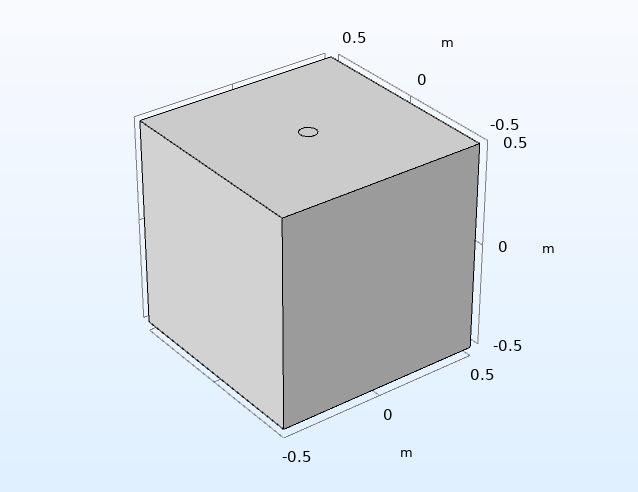
\includegraphics[width=0.8\textwidth]{chapters/chapter4/object.png}
\caption{Geometry of the rock domain with the inserted heated rod.}
\label{fig:comsol_geometry}
\end{figure}

Figure~\ref{fig:comsol_mesh} illustrates the finite element mesh used for solving the coupled thermoelastic problem. The mesh defines both the numerical discretization and the spatial structure later used in graph-based machine learning.

\begin{figure}[h]
\centering
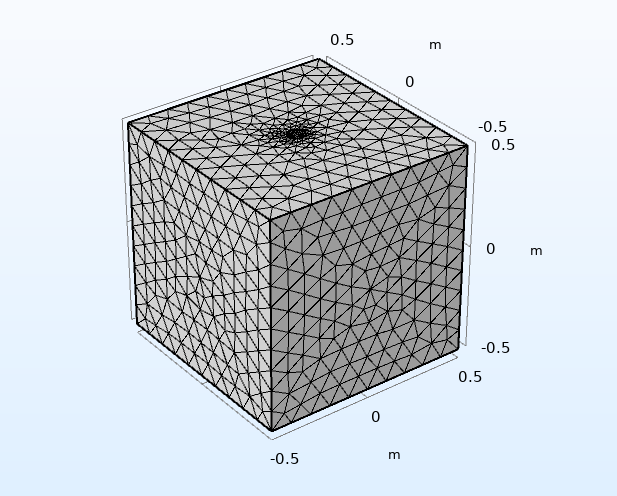
\includegraphics[width=0.8\textwidth]{chapters/chapter4/mesh.png}
\caption{Finite element mesh used for the thermoelastic COMSOL simulation.}
\label{fig:comsol_mesh}
\end{figure}

Figure~\ref{fig:comsol_temperature} shows the temperature distribution produced by the heated rod. This visualization allows checking whether heat propagates from the source into the surrounding rock in a physically reasonable way.

\begin{figure}[h]
\centering
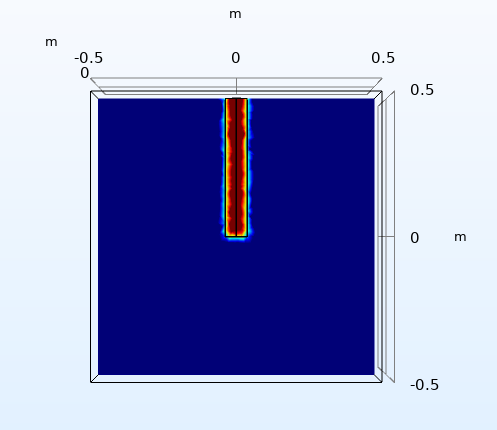
\includegraphics[width=0.8\textwidth]{chapters/chapter4/temperature.png}
\caption{Temperature distribution in the rock caused by the heated rod.}
\label{fig:comsol_temperature}
\end{figure}

Figure~\ref{fig:comsol_stress} shows the stress field generated by non-uniform thermal expansion. This field is important because it represents the mechanical response of the geological medium to the thermal disturbance.

\begin{figure}[H]
    \centering

    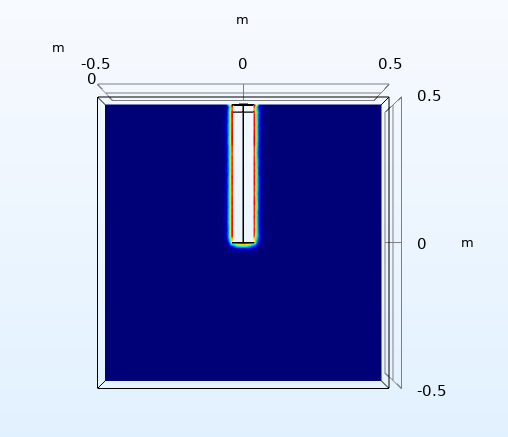
\includegraphics[width=0.8\textwidth]{chapters/chapter4/stress_1.png}

    \vspace{0.3cm}

    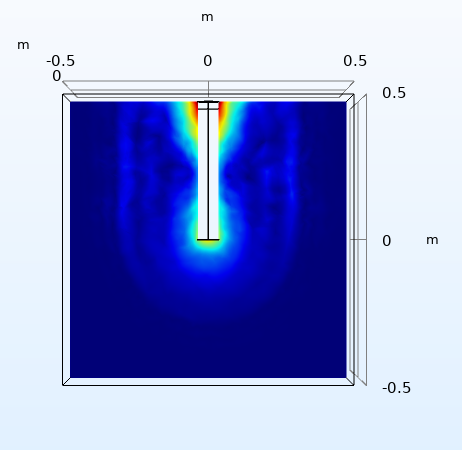
\includegraphics[width=0.8\textwidth]{chapters/chapter4/stress_2.png}

    \vspace{0.3cm}

    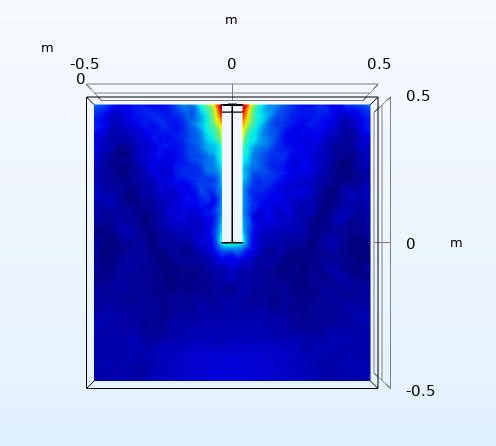
\includegraphics[width=0.8\textwidth]{chapters/chapter4/stress_3.png}

    \caption{Evolution of the stress field in the rock at three time
    instants (top: beginning of the heating; middle: intermediate
    state; bottom: end of the simulated interval). Non-uniform thermal
    expansion produces stress concentrations in the heated zone and
    along the rod--rock interface.}
    \label{fig:comsol_stress}
\end{figure}


\subsubsection{Limitations of the simulation setup}

The quality of synthetic data depends on the geometry, material parameters, boundary conditions, mesh resolution, and solver settings. If the geometry is too simplified, the generated data may not fully represent real geological formations. If the material model assumes homogeneous and isotropic rock, it may differ from real rocks, which can contain cracks, layers, pores, and anisotropic properties.

Mesh resolution also affects numerical accuracy. A coarse mesh may not capture sharp temperature gradients near the rod or stress concentration zones. A very fine mesh improves accuracy, but increases computational cost. Similarly, the selected time step \(\Delta t\) affects stability and accuracy of the time-dependent solution.

Limited computational resources restricted the complexity and number of simulated scenarios. For example, very large two-dimensional models, very fine meshes, and many parameter combinations require significant memory and computation time. However, these limitations were controlled by keeping the setup consistent and by focusing on physically meaningful scenarios.

Despite these limitations, controlled synthetic generation is suitable for training and comparing AI models because all required physical fields are available and consistently exported. This is a major advantage compared to real experimental data, where some fields may be difficult or impossible to measure directly.